\documentclass[tikz,border=3.14mm]{standalone}
\usetikzlibrary{shapes, arrows, positioning, calc}

\begin{document}
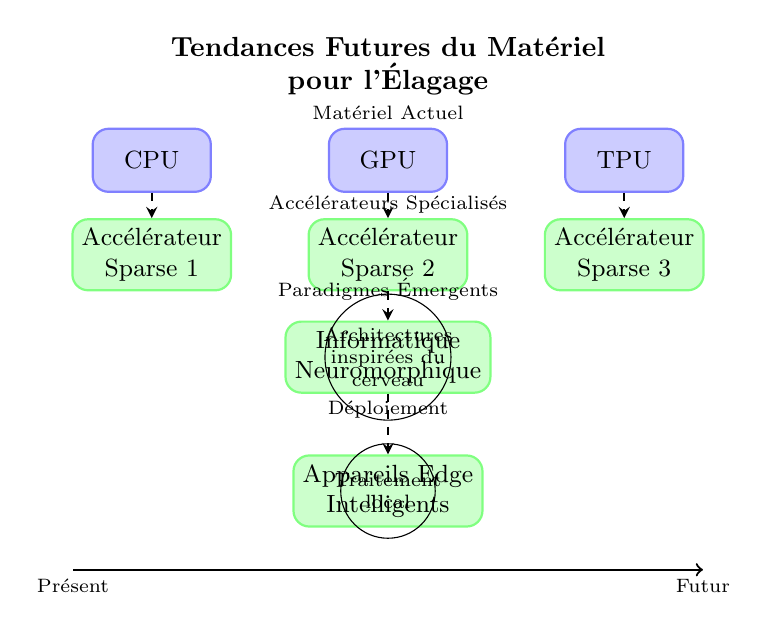
\begin{tikzpicture}[
    node distance=0.8cm,
    component/.style={rectangle, draw=blue!50, fill=blue!20, thick, minimum width=1.5cm, minimum height=0.8cm, rounded corners=0.2cm, align=center, font=\small},
    future/.style={rectangle, draw=green!50, fill=green!20, thick, minimum width=1.5cm, minimum height=0.8cm, rounded corners=0.2cm, align=center, font=\small},
    arrow/.style={->, >=stealth, thick}
]

% Title
\node[align=center, font=\bfseries] at (0, 4.2) {Tendances Futures du Matériel\\pour l'Élagage};

% Current hardware
\node[component] (cpu) at (-3, 3) {CPU};
\node[component] (gpu) at (0, 3) {GPU};
\node[component] (tpu) at (3, 3) {TPU};

% Specialized accelerators
\node[future] (sparse1) at (-3, 1.8) {Accélérateur\\Sparse 1};
\node[future] (sparse2) at (0, 1.8) {Accélérateur\\Sparse 2};
\node[future] (sparse3) at (3, 1.8) {Accélérateur\\Sparse 3};

% Neuromorphic computing
\node[future] (neuro) at (0, 0.5) {Informatique\\Neuromorphique};
\draw (0, 0.5) circle (0.8cm);
\node[align=center, font=\scriptsize] at (0, 0.5) {Architectures\\inspirées du\\cerveau};

% Edge devices
\node[future] (edge) at (0, -1.2) {Appareils Edge\\Intelligents};
\draw (0, -1.2) circle (0.6cm);
\node[align=center, font=\scriptsize] at (0, -1.2) {Traitement\\local};

% Arrows showing evolution
\draw[arrow, dashed] (cpu) -- (sparse1);
\draw[arrow, dashed] (gpu) -- (sparse2);
\draw[arrow, dashed] (tpu) -- (sparse3);
\draw[arrow, dashed] (sparse2) -- (neuro);
\draw[arrow, dashed] (neuro) -- (edge);

% Labels
\node[above, font=\scriptsize] at (0, 3.4) {Matériel Actuel};
\node[above, font=\scriptsize] at (0, 2.2) {Accélérateurs Spécialisés};
\node[above, font=\scriptsize] at (0, 1.1) {Paradigmes Émergents};
\node[above, font=\scriptsize] at (0, -0.4) {Déploiement};

% Timeline
\draw[->, thick] (-4, -2.2) -- (4, -2.2);
\node[below, font=\scriptsize] at (-4, -2.2) {Présent};
\node[below, font=\scriptsize] at (4, -2.2) {Futur};

\end{tikzpicture}
\end{document}